% !TeX spellcheck = en_GB
\section{Experimental Set-up and Procedure}
\subsection{Set-Up}

The experiment was done with a pre-mounted setup as shown in the fig \ref{fig:setup1} with tree main components: Laser source and optical components, electronic and microwave equipment and an Apparatus for NV centre spectroscopy. A reliable radio-frequency system must be deployed, ensuring the microwave-based excitation of the diamonds magnetic resonance. It was important that the oscilloscope and the spectrum analyser to be synchronized to achieve simultaneous optical analysis while sweeping the desired microwaves. A list of the apparatus used in this experiment and also pictures of the set up running can be find in the appendix.

\begin{figure}
	\centering
	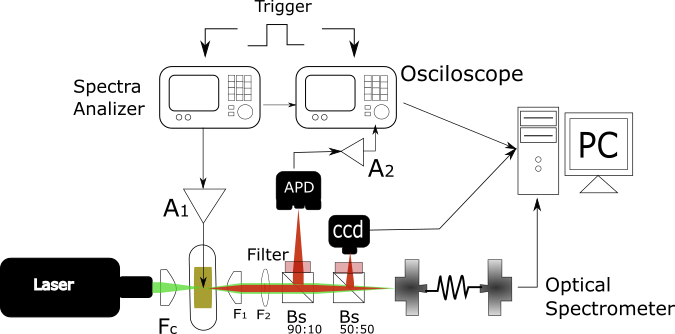
\includegraphics[width=0.7\linewidth]{../figures/setup1}
	\caption[setup]{Schematic not on scales of the experiment. The laser is coupled into an optical fiber and operated via software of Thorlabs. \textbf{Optics}: The laser is focussed on a microstrip (MS) with a condenser lens (Fc). Using a 4-f-system with the lenses f1 and f2 (having focal lengths of 10 and 80 mm, respectively) and a Beam splitting set;with split intensities 10:90 (beampath:APD), and 50:50 (CCD:OS), the diamonds are imaged on an avalanche photo diode (APD), the CCD-camera (CCD) and the optical spectrometer (OS). Low pass Colour filter are added to avoid the pass of the laser.
	\textbf{Electronics}: The output of a spectrum analyser is amplified (amplifier A1, gain = 48) and coupled into the microstrip, which is grounded through an impedance of $50\Omega$.
	The spectrum analyzer and the oscilloscope are triggered with the same signal, recording the data of athe power detector, as well as the amplitude signal (audio amplifier A2) of the APD.  Adapted from \cite{anleitung}.}
	\label{fig:setup1}
\end{figure}

 \subsubsection{Optical set-up}
 
The optical components basically makes a confocal microscope with two lenses ($f1=10\mathrm{mm}$ and $f2=80\mathrm{mm}$) set up at their focal points, forming a 4f-system. A laser of $\lambda=519nm$ was used as illumination source. In the set up an optic fibre had to be couple due lack of space focused with a condenser lend (fc) to the Diamond ins the Microstrip.
In the object plane is the Microstrip \textbf{(Ms)}, in this objective we put a small portion of micro-diamonds powder with a small spire with out touching the strip. The Ms is fundamental to apply the ODMR measurements, a magnet holder is available, which counts with a connector to the spectra Analizer \textbf{(SA)} that supplies the microwaves.

An adjustable mirrors set provides helps to align the laser beam into the strip, giving 3 dimensions to move. For distribute the signal into the Avalanche PhotoDiode \textbf{(APD)} and the ccd camera, Two dicroic mirrors ( acting as beam splitter) was used, one with 90:10 percent and 50:50). The advantage of using a APD is that it providing fast response in time and high sensitivity. Both the CCD and spectrometer are controlled using a computer. To avoid any scattered of light and improve a low signal-background ratio  low pass colour filters \textbf{(CF)} was used after each beam splitter to avoid the laser light to be measure in the data.

\subsubsection{Electronics}

Additionally to the optics, some electronics have to be used to perform the ODMR. First an Oscilloscope is used to read the APD signal after being amplified by an audio amplifies.  As mentioned, a supply of microwaves is couple to the MicroStrip.
Because the transition and reflection in the Ms is unknown an power coupler have was added in the set up show in the next section, so this transmission can be related directly.  To do so, a supply covering the frequency of centre at 2.8GHZ is used, which can be provided by the tracking generator. the SA  was set at 0 dBm and connected to a 45dBm amplified before it reach the Ms as shown in \ref{fig:setup1}.

 A signal generator in square mode trigger the SA and the Oscilloscope in order both measurements coincides so the intensity of the fluorescence detected by the APD can be track immediately the microwaves was imput.
 
 Our tracking generator can sweep through the aforementioned range within 200ms, and  the signal generator was set to ......  Another way to increase the obtained signal is done on the acquisition site: an audio amplifier (A2) also increases the signal provided by the APD, which has previously been filtered using a low pass filter (cut-off frequency fc 100Hz). 
 
 The oscilloscope was used with a build-in phyton software already install in the computer ans slightly modified just in the number of data acquire to 250 loops per measurement.
 
 \subsubsection{Magnets}
 
 Onces the SA and the APD was trigered and the signal was well acquired, one and two magnets was add next to the Microstrip with the purpose of align the Diamond lattice with the magnetic field  and do some measurement respecting this new parameter.
two magnets was used, displayed in a base overpose to the Microstridp and centred to the diamonds powder. The distance between the magnets and the centre was $36 \pm 0.5 \mathrm{mm}$ and several variations was used, including a perpendicular measure in the Z axis and changing of  polarity.  In the next figure a sketch of the base used is shown as the axis of the lab reference.
\begin{figure}
	\centering
	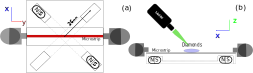
\includegraphics[width=0.7\linewidth]{../figures/magnets}
	\caption[mag]{top and side view of the magnet base over the microstrip, The magnets was put in the strips of the base alwasys at the same distance, the reference of the axis are respective the laboratory frame.}
	\label{fig:magnets}
\end{figure}


\subsection{Calibration}

\subsubsection{conversion factor camera}

The length of the strip was measured with a calliper at $1.2\pm 0.1\mathrm{mm}$ and the camera used was a Thorlabs CCD camera had dimensions of 1280x1024 pixels, each pixel with $5.2\times5.2 \mathrm{\mu m}$ according to the manufacturer.
In order to know the actual resolution of our microscope a calibration was done based on the magnification and calibration factor of the set up.
Theoretically our $C_{f}$ can be calculated from the lenses $f_{1}$ and $f_{2}$ that gives a Magnification of 8. The calibration factor is given by:
\\

\begin{equation}
C_{f}=\dfrac{1 px \cdot M}{d_{p}} = 1552 px/mm
\end{equation}\\

Where $M$ is the magnification and $d_{p}$ is the pixel sizes.

For getting an experimental magnification we measure the distance in pixel of or strip using the the tool of Thorlab’s software and overlapping two pictures as shown in fig \ref{fig:distance-sslip}. The strip had in total 1442 pixels of cross section  with leads to  a magnification factor close to $M=7$.
Using the equation above and the respective measurement we denote that the  $C_{f} =1346\pm224 \,\mathrm{px/mm}$,
 \begin{figure}
 	\centering
 	\includegraphics[width=0.7\linewidth]{"../figures/distance sslip"}
 	\caption{Overlay of the two pictures that shows the wide of the strip using a bright diamond in the centre as a reference point. The measurements was done insitu but the  images overlay was done with FIJI software in a post analysis.}
 	\label{fig:distance-sslip}
 \end{figure}
 

\subsubsection{Laser Power}
To set the power of the laser to a reasonable value a calibration curve was recorded which shows the actual laser power at the position of the Ms plotted over the output power set in the GUI. This curve is shown in figure \ref{fig:power}.\\

Using this graph the output power was set to $P_\text{out}=20\,\mathrm{mW}$ which corresponds to an actual laser power of $P_\text{act}=(27.4\pm1.4)\,\mathrm{mW}$.
\begin{figure}[hb]
	\centering
	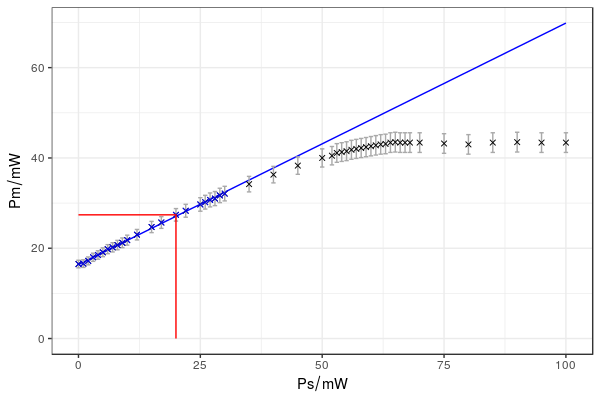
\includegraphics[width=0.65\textwidth]{../figures/powercal.png}
	\caption{Measurement of the laser power}
	\label{fig:power}
\end{figure}


\subsubsection{Electronic components}


In order to perform our ODMR measurements it is crucial to determine the amount of microwave power deployed into the microstrip and the diamonds. We can not know the absolute power that is plugged in. The micro strip by default have some transition $T_{Ms}$ and reflections $R_{Ms}$ that we need to measure experimentally.
For this, a power coupler was added to the set-up and four measurement with different arranges where performed as shown in the fig. \ref{fig:apd}.
First, the power coupler (PC) was connected to the DSA in out- out position to know the it´s transmission, $T_{cpl}$. On the other hand the second set-up, an In- Out connection to the SA to determine the reflection of the CPL $R_{cpl}$. For the third and fourth display, the Ms was added, in the Out-Out position (CPL-DSA), measuring the Reflection $R_{cpl-Ms}$ and transmission $T_{cpl-Ms}$ of the hole set.


\begin{figure}[hb]
	\centering
	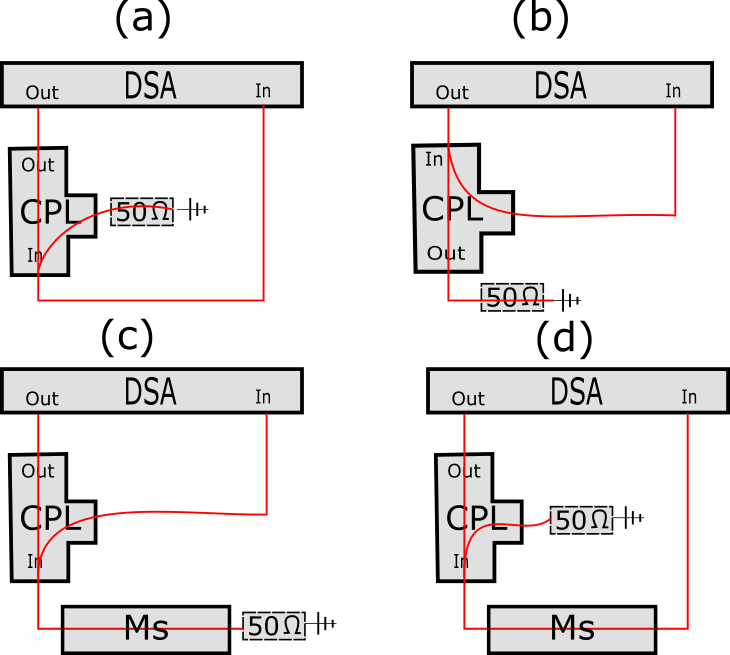
\includegraphics[width=0.7\linewidth]{../figures/APD}
	\caption[Diferent arranges of the CPL and MicroStrip conected to the DSA]{(A) Power coupler connected to the SA in Out-Out direction measuring $T_{cpl}$, (b) Cpl connected in Out-In sequence and measuring $R_{cpl}$, (c) CPl and micro strip connected in Out-Out mode and measuring the $R_{cpl-Ms}$ (d) CPL and Microstrip connected in Out-Out mode and measuring $T_{cpl-Ms}$}
	\label{fig:apd}
\end{figure}

The SA was set at 0 Dbm with a sweep centred at 2.8GHz frequency. A 50$\Omega$ resistance was used for the losses ends as shown. The next figure display the four signals of the different arranges.

\begin{figure}
	\centering
	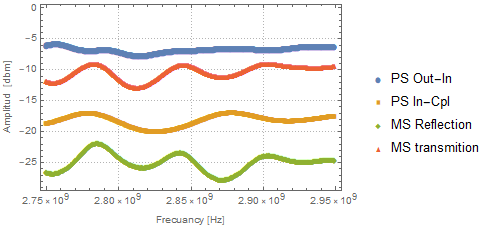
\includegraphics[width=0.7\linewidth]{../figures/microstrip}
	\caption{Attenuation od the power at 0dBm from top to bottom: $T_{CPL}$,$T_{Cpl-Ms}$, $R_{CPL}$ and $R_{Cpl-MS}$}
	\label{fig:microstrip}
	\end{figure}

The total transmission and reflection was simply calculated by a subtraction of the Ms transmission in the different processes as next.

\begin{align}
T_{Ms}&=T_{cpl-Ms}-T_{cpl}\\
R_{MS}&=R_{cpl-Ms}+T_{cpl}-R_{cpl}
\end{align}


The attenuation in this cases for the transmission remains close to cero, specially in the centre of the sweep while the reflection as shown reduces drastic. This gives us the idea that the power transmitted is close to the 0dBm used in the SA and few of it is been reflected.

\begin{figure}
	\centering
	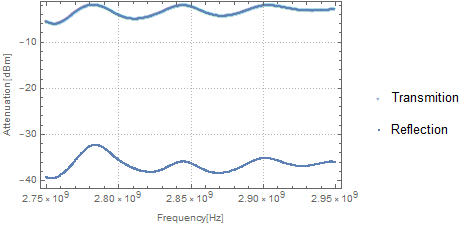
\includegraphics[width=0.7\linewidth]{../figures/microstrip-trasm-eflect}
	\caption[trans-refl]{Attenuation of the resultant transmission (top) and reflection (bottom) at the Microstrip, at 0dBm in a 2.8GHZ frequency centre.}
	\label{fig:microstrip-trasm-eflect}
\end{figure}

\subsubsection{Optical Spectrometer}
The optical spectrometer is later used to record the fluorescence spectrum of the diamond. To calibrate the optical spectrometer we first record the spectrum of visible light and compare the identified Fraunhofer lines with their literature values. The recorded spectrum is shown in figure \ref{fig:sunspectrum} and the values are given in table \ref{tab:fraunhofer}.\\

Since only small statistical deviations in both directions could be found there was no need to calculate a conversion factor and the values given from the optical spectrometer were verified. \\

The optical spectrometer was also used to get the actual wavelength of the laser which was determined in figure \ref{fig:laserspectrum} to be $\lambda=(517.3\pm0.2)\,\mathrm{nm}$.
\begin{figure}
	\centering
	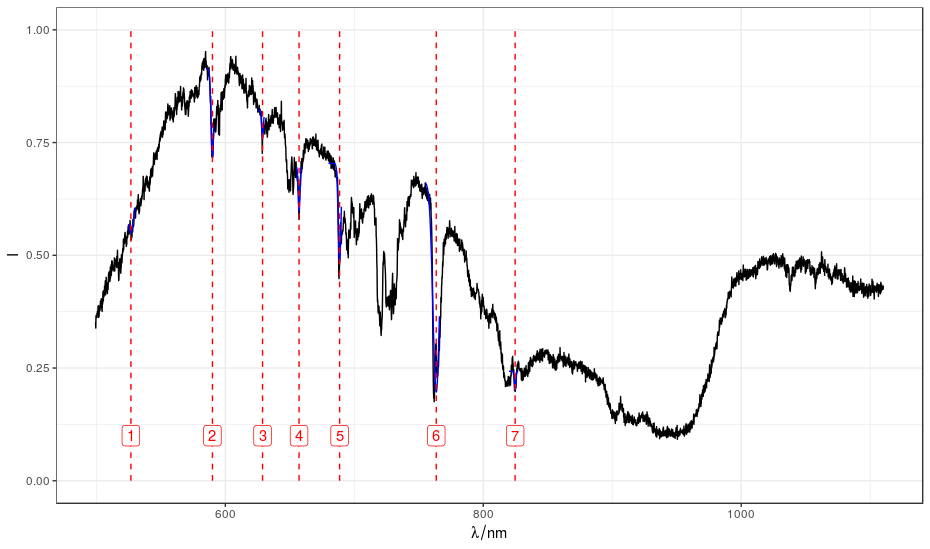
\includegraphics[width=0.8\textwidth]{../figures/sunspectrum.png}
	\caption[Spectrum of the sun with identified Fraunhofer lines]{Spectrum of the sun with identified Fraunhofer lines for calibration of the optical spectrometer}
	\label{fig:sunspectrum}
\end{figure}

\begin{table}
	\centering
	\begin{tabular}{c|c|c|c|c}
		Peak&Position&Element&Position \cite{fraunhoferlines}&Difference\\
		1&$526.8\pm1.7$&Fe I&527.0&$-0.2$\\
		2&$590.0\pm0.5$&Na I&589.6&$+0.4$\\
		3&$628.9\pm0.3$&Fe I&630.3&$-1.4$\\
		4&$657.2\pm0.3$&H $\alpha$&656.3&$+0.9$\\
		5&$688.6\pm0.5$&&&\\
		6&$763.5\pm1.3$&&&\\
		7&$824.7\pm0.3$&&&\\
	\end{tabular}
	\caption{Positions of the Fraunhofer Lines compared to the literature values}
	\label{tab:fraunhofer}
\end{table}

\begin{figure}
	\centering
	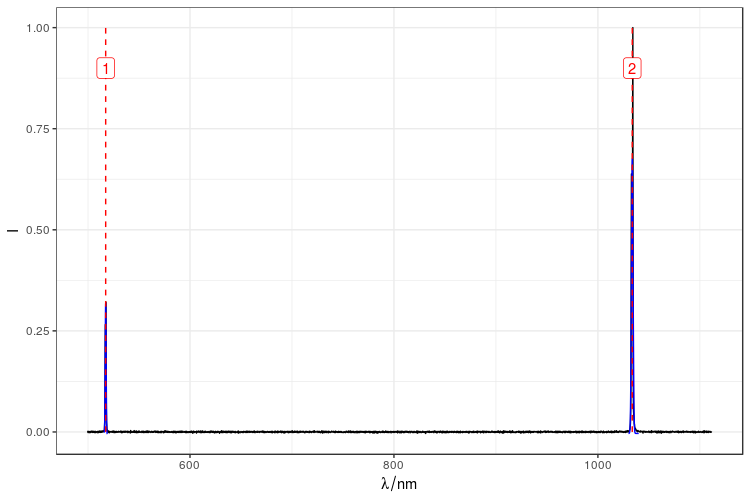
\includegraphics[width=0.8\textwidth]{../figures/laserspectrum.png}
	\caption[Spectrum of the laser]{Spectrum of the laser with identified peaks at the wavelengths $\lambda=(517.3\pm0.2)\,\mathrm{nm}$ and $\lambda=(1033.7\pm0.4)\,\mathrm{nm}$}
	\label{fig:laserspectrum}
\end{figure}

\subsubsection{ODMR calibrations}
\label{sec:odmr-cal}
\paragraph{Shielding}
To improve the ODMR signal and avoid noise generated by the microwaves a shielding cage was built around the APD. In figure \ref{fig:odmr-shield} the effect of this shielding cage on the ODMR spectrum is shown.
\begin{figure}
	\begin{subfigure}{0.5\textwidth}
		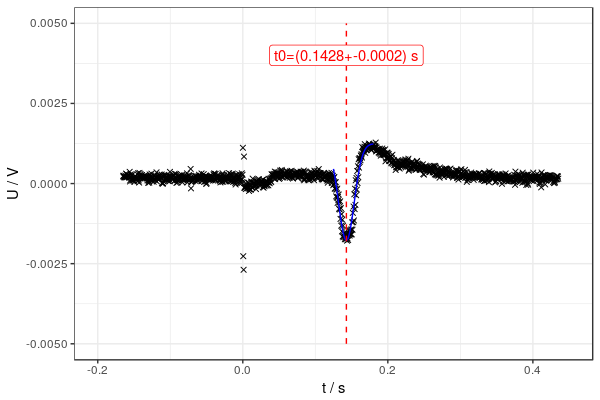
\includegraphics[width=\textwidth]{../figures/odmr-cal-1.png}
		\subcaption{without shielding}
	\end{subfigure}
	\begin{subfigure}{0.5\textwidth}	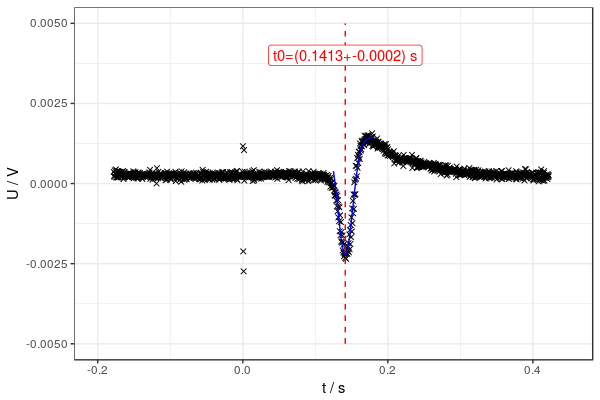
\includegraphics[width=\textwidth]{../figures/odmr-cal-2.png}
		\subcaption{with shielding}
	\end{subfigure}
	\caption{ODMR spectrum}
	\label{fig:odmr-shield}
\end{figure}
\paragraph{Time-to-Frequency Conversion}

\begin{figure}
	\begin{subfigure}{0.5\textwidth}
		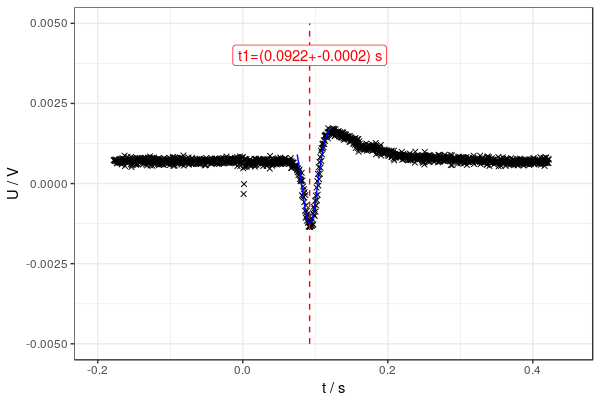
\includegraphics[width=\textwidth]{../figures/odmr-cal-4.png}
		\subcaption{shifted to the left}
	\end{subfigure}
	\begin{subfigure}{0.5\textwidth}
		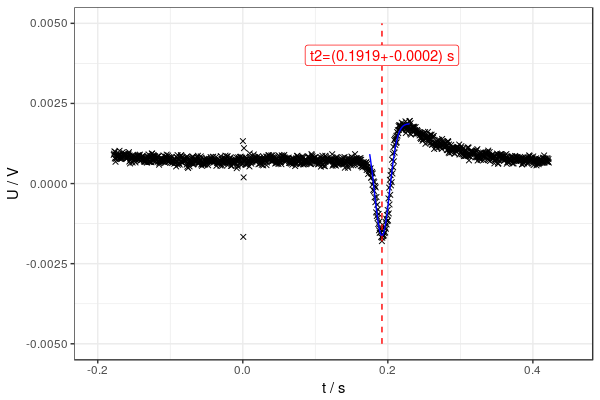
\includegraphics[width=\textwidth]{../figures/odmr-cal-3.png}
		\subcaption{shifted to the right}
	\end{subfigure}
	\caption{ODMR spectrum for time-to-frequency calibration}
	\label{fig:odmr-shift}
\end{figure}

Performing ODMR measurements we achieve the ODMR spectra on the oscilloscope. Therefore the spectra are time-resolved. To gain frequency-resolved spectra we need to calculate the conversion factor from time to frequency. We do this by performing two sweeps with shifted centre frequencies which allows us to calculate the conversion factor and also the offset since we know the frequency at which the peak appears.

The conversion can be expressed by the following equation:

\begin{align}
f(t)&=\frac{f(t_1)(t_1-t_2)-(f(t_1)-f(t_2))t_1}{t_1-t_2}+\frac{f(t_1)-f(t_2)}{t_1-t_2}\cdot t
\end{align}

Inserting the values achieved from figure \ref{fig:odmr-shift} we get the following conversion function:

\begin{align}
f(t)&=(1.003\pm0.003)\,\mathrm{\frac{GHz}{s}}\cdot t+(2.728\pm0.011)\,\mathrm{GHz}
\end{align}

Later in this document all spectra are converted by this function and therefore shown in the frequency domain. The errors are gained from the fit and propagated using Gaussian error propagation.

\subsection{Measurements}